\section{Methods}
\begin{figure*}[ht!]
	\centering
	
\includegraphics[width=0.79\linewidth]{figure/model.pdf} % Reduce the figure size so that it is slightly narrower than the column.
	\caption{The overall structure of our method. We adopt Faster RCNN as the object detector. Dual Transformer is used to encode object/relationship features. RTPB addresses the long-tail problem by adjusting the classification logits of each relationship.}
	\label{fig:model}
\end{figure*}
\subsection{Problem Setting and Overview}
\subsubsection{Problem Setting}
Given an image $\mathcal{I}$, our goal is to predicate a graph $\mathcal{G} = \{\mathcal{V},\mathcal{E}\}$, where $\mathcal{V}$ is the set of objects in the image and $\mathcal{E}$ is pairwise relationships of objects in $\mathcal{V}$. Each object $v \in \mathcal{V}$ consists of the bounding box coordinates $\textbf{\textit{b}}_v$ for location and the class label $c_v$ for type. An edge $e \in \mathcal{E}$ should include the pair of a subject and a object, \textit{i.e.}, $(v_s, v_o)$,  and the label of the relationship $r$ between $v_s$ and $v_0$.
% Typically, most current SGG models including our method are optimized in a supervised way. Thus the types of objects are limited in a set $\mathcal{C}_e$ of types and the categories of relationships are limited in a set $\mathcal{C}_r$ of relationship types.
Typically, for object $v\in \mathcal{V}$, the label  $c_v$ belongs to $\mathcal{C}_e = \{1,2,...,L_e\}$, where $L_e$ is the number of object labels. The label of relationship $c_r$ are in $\mathcal{C}_r = \{1,2,...,L_r\}$, where $L_r$ is the number of relationship labels. 
\par In the commonly used SGG pipeline, the probability of scene graph $Pr(\mathcal{G}|\mathcal{I})$ is formulated as follows
\begin{equation}
  Pr(\mathcal{G}|\mathcal{I}) = Pr(\mathcal{B}|\mathcal{I})Pr(\mathcal{O}|\mathcal{I},\mathcal{B})Pr(\mathcal{G}|\mathcal{I},\mathcal{B}, \mathcal{O}),  
\end{equation}
where $ Pr(\mathcal{B}|\mathcal{I})$ indicates the proposal generation. The $\mathcal{B}$ is the set of bounding box $b_v$, which is conducted by an object detector. $Pr(\mathcal{O}|\mathcal{I},\mathcal{B})$ denotes the object classification. The $\mathcal{O}$ is the set of object class $c_v$, and $Pr(\mathcal{G}|\mathcal{I}, \mathcal{B}, \mathcal{O})$ means the final relationship classification.

\subsubsection{Methods Overview}
Figure \ref{fig:model} shows the overall structure of our method. Following previous works \cite{Tang2020_unbiased,Zellers_2018_CVPR}, we utilize Faster RCNN \cite{ren2015faster} to generate object proposals and the corresponding features from the input image.
For each object proposal, the object detector conducts the bounding box coordinates 
$\textbf{\textit{b}}_v$, %\in\mathbb{R}^4%
the visual feature 
$\textbf{\textit{g}}_v$,
and the object classification score $\textbf{\textit{z}}_v\in\mathbb{R}^{|\mathcal{C}_v|}$.
Besides, to improve the relationship prediction, the backbone also generates the feature of the union boxes of each pair of objects.
Then, we introduce our \textit{Dual Transformer (DTrans)}, which uses two stacks of Transformers to encode the context-aware representations for objects and relationships, respectively (see Section \ref{sec:DTrans}). Moreover, to address the long-tail problem for SGG, we adopt the \textit{\textbf{r}esistance \textbf{t}raining using \textbf{p}rior \textbf{b}ias (RTPB)} for unbiased SGG. The RTPB assigns resistance to the model by the prior bias, named resistance bias (see Section \ref{sec:RTPB}).
% In this work, we adopt resistance training using prior bias (RTPB) and a dual transformer structure (DTrans) for the scene graph generation:
% 1) The RTPB assigns resistance to the model by the prior bias, named resistance bias, to address the imbalance problem. (Section \ref{sec:RTPB})
% by adjusting the training process and the classification boundary based on the prior statistic about the imbalanced training set.
% 
% The resistance bias module is initialized with data from the training set or other prior data in the model building phase. Based on these prior data, the bias module conducts a bias value for each class of relationship. Then the module provides an extra bias item for the relationship classifier in the training phase to manually adjust the classification boundary and keeps silent in the evaluation phase.
% 2) The Dual Transformer uses two stacks of transformers to encode the global features for objects and relationships, respectively. (Section \ref{sec:DTrans})

% \begin{equation}
% 	\mathbf{v} = \{\mathbf{b}_v, \mathbf{g}_v, c_v\},
% \end{equation}

\subsection{Dual Transformer}
\label{sec:DTrans}
% The RTPB improves the SGG performance by proper head-tail trade-off for the relationship classification. To achieve better performance, it's still necessary to conduct better features of the relationship. And we address this problem by
We propose the Dual Transformer (DTrans) for better contextual information encoding. As shown in Figure \ref{fig:model}, based on the outputs of the object detector, i.e., the location of objects, the feature of objects, and the feature of union boxes, the DTrans uses self-attention to encode the context-aware representation of objects and relationships.
% refine the classification results of objects and recognize the relationships between these objects.
%

\subsubsection{Self-attention}
Our model uses two stacks of transformers to obtain the contextual information for objects and the corresponding pairwise relationships. Each transformer encodes the input features with self-attention mechanisms \cite{vaswani2017attention}, which mainly consists of the attention and the feed-forward network. The attention matrix is calculated as
\begin{equation}
	Attention(Q,K,V) = \sigma(\frac{QK^T}{\sqrt{d_k}})V,
\end{equation}
where query ($Q$), keys ($K$), and value ($V$) are obtained from the input feature through three different linear transformation layers, $1/\sqrt{d_k}$ is the scaling factor for the dot product of $Q$ and $K$~\cite{vaswani2017attention}, and $\sigma$ is the softmax function. Besides, we utilize the multi-head attention, which is used to divide the Q, K, and V into $n_h$ parts and calculates the attentions of each part. Next, a feed-forward network (FFN) is used to mix the attentions of each part up.

\subsubsection{Object Encoder}
As shown in Figure \ref{fig:model}, based on all the results about object proposals from the object detector, we first compose them to initialize a feature vector of the corresponding object as follows:
\begin{equation}
	\mathbf{e}_v = W_o[pos(\textbf{\textit{b}}_v),\textbf{\textit{g}}_v, ebd(c_v)],
\end{equation}
where $[\cdot,\cdot]$ denotes the concatenation operation, the $pos$ is a learnable position encoding method for object location, $ebd(c_v)$ is the GloVe vector embedding for object label $c_v$, and $W_o$ is a linear transformation layer used to initialize the object feature from the above information. 
Then, we feed the $\mathbf{e}_v$ into a stack of $n_o$ transformers to obtain the final context-aware features $\mathbf{e}_v^{final}$ for objects. 
The $\mathbf{e}_v^{final}$ is first used to produce the final classification result of objects as follows:
\begin{equation}
    \mathbf{p}_v = \sigma(W_{clf}^{o}\mathbf{e}_v^{final}),
\end{equation}
where $W_{clf}^{o}$ is the object classifier. 
And then, the $\mathbf{e}_v^{final}$ is also used to generate the features of the pairwise relationships of objects.
% Then, we feed the feature of objects into the transformer encoder as follows:
% \begin{equation}
%     \mathbf{e}_v^{final} = encoder(\mathbf{e}_v)
% \end{equation}

\subsubsection{Relationship Encoder}
% \subsubsection{Feature Fusion}
Before encoding the features of relationships, we first carry out a feature fusion operation to generate the basic representation of relationships. For each directed object pair $(s,o)$, we concatenate the visual feature $\mathbf{g}_{U(s,o)}$ of the union box of $s$ and $o$, and the context-aware features of the subject $s$ and the object $o$. Then, we use a linear transformation to obtain the representation of the relationship between the subject $s$ and the object $o$:
% to generate the representation of the relationship between subject $s$ and object $o$.
\begin{equation}
	\mathbf{e}_{s,o} = W_r[\mathbf{g}_{U(s,o)},\mathbf{e}_s^{final}, \mathbf{e}_o^{final}],
\end{equation}
where $W_r$ is a linear transformation layer used to compress the relationship features. $\mathbf{e}_s^{final}$ and $ \mathbf{e}_o^{final}$ are the final context-aware features of subject $s$ and object $o$.

Then, we use another stack of $n_r$ Transformers to encode the features of relationships and produce the final feature $\mathbf{e}_{s,o}^{final}$ for the relationship between subject $s$ and object $o$. Finally, the relationship classifier uses the feature $\mathbf{e}_{s,o}^{final}$ to recognize the pairwise relationships as follows
\begin{equation}
	\mathbf{p}_{s,o} = \sigma(\mathbf{z}_{s,o}) = \sigma(W_{cls}^r\mathbf{e}_{s,o}^{final}),
	\label{eq:p}
\end{equation}
where $\mathbf{z}_{s,o} = W_{cls}\mathbf{e}_{s,o}^{final}$ is  vector of the logits for relationship classification, and$W_{cls}^r$ is the relationship classifier.
% If apply our RTPB, the relationship prediction turns to be 
% \begin{equation}
%     \mathbf{p}_{s,o} = \sigma(\mathbf{Z}_{s,o} + \mathbf{b}) = \sigma(W_{cls}\mathbf{e}_{s,o}^{final} + \mathbf{b}),
% \end{equation}
% where $\mathbf{b} = [b_1,b_2 .., b_{\|\mathcal{C}_r\|}]$ consists of the resistance bias value for each relationship in $\mathcal{C}_r$, and $b_i$ indicate the resistance bias value for $i-th$ relationship in $\mathcal{C}_r$.

\subsection{Resistance Training using Prior Bias}
\label{sec:RTPB}
%In scene graph generation, one of the most important tasks is to recognize the relationships between objects. Thus it's vital 
% Resistance bias takes the advantage of the FREQ proposed by \citeauthor{Zellers_2018_CVPR}(2018). The FREQ act as a default value of the logits classification score. We further study its impact on the model and find out that the FREQ encourage the rest model to conduct the result with different distribution to the bias.  
%the distribution statistics of the training set can provide more valid information, like the long-tail distribution. 
Inspired by the idea of resistance training that muscle turns to be stronger if they are training with heavier resistance \cite{kraemer2004fundamentals},
we propose the resistance training using prior bias (RTPB) for unbiased SGG. Our RTPB uses the prior bias as the resistance for the model only during training to adjust the model's strength for different relationships. We name the prior bias as resistance bias, which is applied to the model in the training phase as:
% module to use the prior information to adjust the training phase for obtaining an unbiased SGG model. The resistance bias is similar to the FREQ baseline but only for the training phase in most situations. 
%To achieve this target, we conduct the bias item $b_r$ for each relationship and use it as follows:
\begin{equation}
	\hat{\mathbf{z}}_{s,o} = \mathbf{z}_{s,o} - \mathbf{b},
\end{equation}
% where $i\in\mathcal{C}_r$ is the relationship, the $z_i$ is the logits classification scores for relationship $i$ between subject $s$ and object $o$, and the $b_i$ is the resistance bias for relationship $i$. 
where $\mathbf{z}_{s,o}= [z_1,z_2,...,z_{L_r}]$ is the vector of logits for relationship classification in Eq. \eqref{eq:p}, and $\mathbf{b} = [b_1, b_2,...,b_{L_r}]$ is the vector of resistance bias for each relationship. 
% The $\hat{\mathbf{z}}_{s,o}$ will replace the $\mathbf{z}_{s,o}$ and be used in the classification of relationship.
% The bias $\mathbf{b}$ put resistance on the model to strengthen the corresponding part of the model during training.
By assigning relatively heavier resistance to the tail relationships during training, we enable the model without resistance to handle the tail relationships better and obtain a balanced performance between the tail relationships and the head relationships.
% Because we need the model to pay more effort in dealing with the tail relationships, the head relationships should be corresponding to smaller resistance bias while the tail relationships correspond to larger resistance bias.

In the following part of this section, 
we first introduce four resistance biases from the prior statistic about the training set. Then, we analyze how RTPB works through the loss and the objective.
% For those rare relationships, there will be large resistance to 
% By applying the prior bias corresponding to the training data distribution, we significantly alleviate the bias effect of the imbalanced data and obtain a balanced scene graph generation model.
\subsubsection{Instances for Resistance Bias}
% Now that we know the effect of the RTB module, to address the long-tailed problem with resistance, we need to initialize the bias value corresponding to the distribution of training set to resist the impact of uneven distribution. In this way, we can implement transactions from the head class to the tail one.
\par We define the basic form of resistance bias $b_i$ for relationship $i \in \mathcal{C}_r$ as follows:
\begin{equation}
	b_i = -log \left(\frac{w_i^{a}}{\sum_{j \in \mathcal{C}_r} w_j^a}+ \epsilon\right),
	\label{eq:bias}
\end{equation}
where $w_i$ is the weight of relationship $i$, and $a$, $ \epsilon$ are the hyper-parameters used to adjust the distribution of $b_i$. For resistance bias, the category weight $w_i$ is negatively correlated to the  resistance bias value $b_i$. Therefore, to assign the head categories of relationship small resistance, the distribution of the weight $w_i$ should be correlated to the long-tail distribution of the training set. We introduce four resistance biases:



\textit{\textbf{C}ount Resistance \textbf{B}ias (\textbf{CB})} Intuitively, for the general classification task, we can set the bias weight $w_i$ of resistance bias with the proportion of sample for each relationship in the training set. We denote this type of resistance bias as \textbf{c}ount resistance \textbf{b}ias (CB).  
% The weight $w_i$ is set as the proportion of relationship $i$ in the training set.
% the count of relationship $i$ in the training set.

\textit{\textbf{V}alid Resistance \textbf{B}ias (\textbf{VB})} 
Besides the number of samples, the long-tail problem also occurs between the general descriptions and the detailed ones. 
% Therefore, we take the count of pair $(s,o)$ for each relationship into consideration. 
Therefore, we formulate valid pair as follows: 
if there is relationship $i\in \mathcal{C}_r$ for object pair $(s,o)$ in the training set, the $(s,o)$ is a valid pair of relationship $i$. 
The distribution of valid pair count for the popular SGG data set, Visual Genome \cite{krishna2016visual}, is shown in the Figure.\ref{fig:dist}. We set the weight $w_{i}$ as the proportion of valid object pair for relationship $i$. In this way, the RTPB can distinguish between the general descriptions of relationships and the rare ones. We call this resistance bias \textbf{V}alid Resistance \textbf{B}ias (VB for short).

\textit{\textbf{P}air Resistance \textbf{B}ias (\textbf{PB})} However, for the SGG task, the classification of relationship is related to not only the relationship, but the pair of entities. Thus we try to use the relationship distribution of each object pair. For different object pairs, the bias are different. In application, we select the bias based on the classification result of objects. For object pair $(s,o)$, the resistance bias for relationship $i$ is follows:
\begin{equation}
    b_{s,o,i} = -log \left(\frac{w_{s,o,i}^{a}}{\sum_{j \in \mathcal{C}_r} w_{s,o,j}^a}+ \epsilon\right),
    \label{rtpb:eq:bsoi}
\end{equation}
where $w_{s,o,i}$ s the ratio of the relationship $i$ in all the relationships between subject $s$ and object $o$ in the training set. And we call this resistance bias as \textbf{P}air Resistance \textbf{B}ias (PB)

\textit{\textbf{E}stimated  Resistance \textbf{B}ias (\textbf{EB})}  Because many pairs of $s,o$ have only a little number of valid relationships and few annotations, the number of relationship sample for particular object pair can hardly show the general distribution of relationship in many cases. Thus we propose subject-predicate and predicate-object count $n^{sppo}$ to estimate the relationship distribution. For subject $s$, object $o$ and relationship $i$, it's calculated as
\begin{equation}
	n_{s,o,i}^{sppo}  = \sqrt{\sum_{o' \in \mathcal{C}_e}{n_{s,o',i}}\times \sum_{s' \in \mathcal{C}_e}{n_{s',o,i}}},
\end{equation}
where $n_{s,o,i}$ is the count of relationship $i$ between subject $s$ and object $o$. Then we produce a new resistance bias by replacing the weight $w_{s,o,i}$ in Eq.\eqref{rtpb:eq:bsoi} with the proportion ${n_{s,o,i}^{sppo}}/{\sum_{j \in \mathcal{C}_r}{n_{s,o,j}^{sppo}}}$.
% follows:
% \begin{equation}
%     w_{s,o,i} = \frac{n_{s,o,i}^{sppo}}{\sum_{j \in \mathcal{C}_r}{n_{s,o,j}^{sppo}}}.
% \end{equation}
We name this type of resistance as \textbf{E}stimated  Resistance \textbf{B}ias (EB)

\begin{figure}[t]
	\centering
	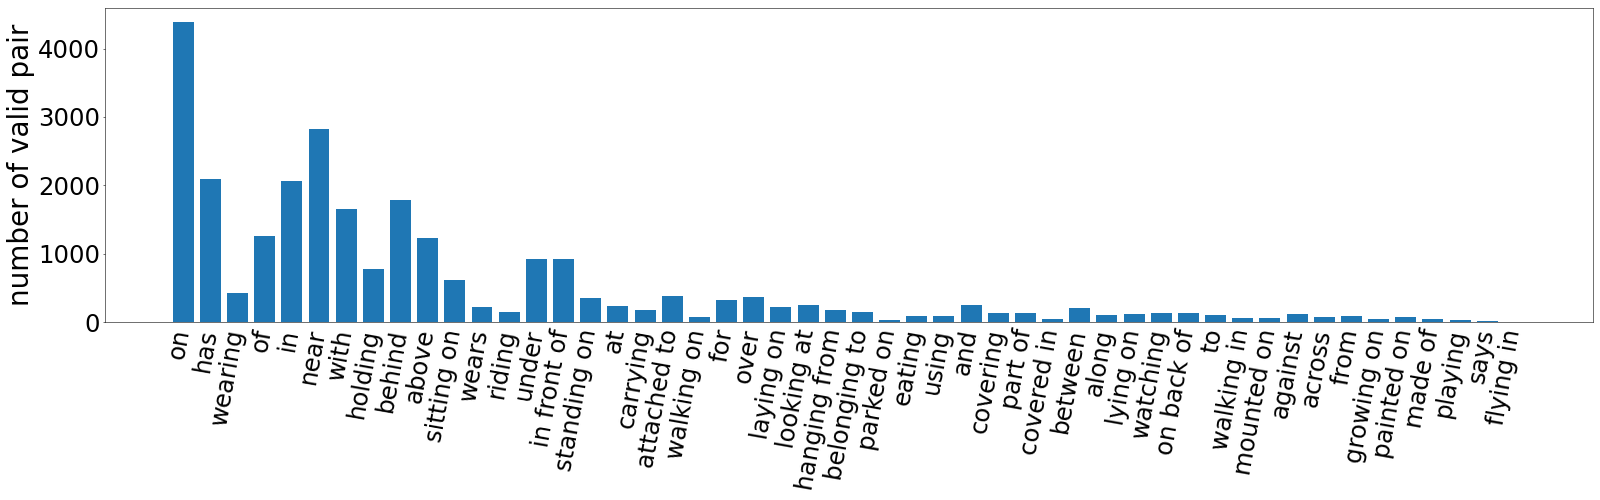
\includegraphics[width=0.99\columnwidth]{figure/valid_pair_dist.png} % Reduce the figure size so that it is slightly narrower than the column.
	\caption{The distribution of the valid pair count.}
	\label{fig:dist}
\end{figure}


% \textit{Mixed resistance bias (MB)}
% We also attempt to take advantage of both CB and PB, and propose the \textbf{m}ixed resistance \textbf{b}ias (MB).
% \begin{equation}
% 	b_{i}^{MB} = \frac{1}{2}b_{i}^{CB}+ \frac{1}{2}b_{i}^{PB},
% \end{equation}
% where $b_{i}^{CB}$ and $b_{i}^{PB}$ are the count resistance bias and valid pair resistance bias for relationship $ i \in \mathcal{C}_r$.
% % We carry out experiments of three SGG sub-task with those resistance bias instances to verify their efficiency. 
% Moreover, we have also tried several other instances of resistance bias, and we will introduce them in Section \ref{sec:otherIns}.
% For convenient, let the probability without RTB be $p_i = Pr(r_i|s,o,I)$
\subsubsection{Loss with RTPB}
In this section, we analyze the effect of RTPB through classification loss. In the classifier, we conduct the final relationship classification probability by a softmax function, and we use the cross-entropy (CE) to evaluate the classification optimization objective. 
%For example, the original probability without RTPB that the relationship between object pair $(s,o)$ in image $\mathcal{I}$ is $i$ , 
The  classification probability and CE loss are shown in follows,
% \begin{equation}
%     \mathcal{L}_i = -log(p_i) = -log \frac{e^{z_{i}}}{\sum_{j\in \mathcal{C}_r}e^{z_{j}}},
%     \label{eq:p_i}
% \end{equation}
\begin{align}
 p_i & = Pr(i|s,o,\mathcal{I}) = \sigma (\mathbf{z}_{s,o})_i = \frac{e^{z_{i}}}{\sum_{j\in\mathcal{C}_r}e^{z_{j}}}, \label{eq:p_i}\\
\mathcal{L}_i & = -log(p_i) = -log \frac{e^{z_{i}}}{\sum_{j\in \mathcal{C}_r}e^{z_{j}}}, \label{eq:l_i}
\end{align}
where $p_i$ is the probability that the relationship between object pair $(s,o)$ in image $\mathcal{I}$ is $i$, and $\mathbf{z}_{s,o} $is the vector of logits for relationship classification mentioned in Eq. \eqref{eq:p}. If we apply our RTPB, the probability $p_i$ in Eq. \eqref{eq:p_i} turns to be:
\begin{equation*}
	\hat{p}_i = \sigma ({\mathbf{z}}_{s,o} - \mathbf{b})_i = p_i\frac{e^{ -b_{i}}}{\sum_{j\in \mathcal{C}_r}e^{-b_{j}} p_j},
\end{equation*}
where $\mathbf{b}= [b_1,b_2,...,b_{L_r}]$ is vector of resistance bias.
% By default, the softmax cross-entropy used to evaluate the classification optimization objective is defined as:
% \sigma(\mathbf{Z}_{s,o})_i
% where the i is the ground-truth relationship between corresponding object pair.
And the softmax cross-entropy loss turns to be:
% \begin{equation}
% 	\begin{split}
% 		\mathcal{\hat{L}}_i 
% 		& = -log(\hat{p}_i)
% 		  = -log \frac{e^{z_{i} - b_{i}}}{\sum_{j\in \mathcal{C}_r}z_{j} - b_{j}}\\
% % 		& = -log \frac{e^{z_i}}{\sum_{j\in \mathcal{C}_r}e^{z_j}} \frac{e^{-b_{i}}{\sum_{j\in \mathcal{C}_r}e^{z_j}}}{\sum_{j\in \mathcal{C}_r}e^{z_j-b_{j}}}\\
% 		%		& = -log Pr(i|s,o,I) - b_{s,o,i}  + log \sum_{j\in \mathcal{C}_r}e^{b_{s,o,j}} Pr(j|s,o,I)\\
% 		& = -log \frac{e^{z_i}}{\sum_{j\in \mathcal{C}_r}e^{z_j}} + b_i + log \sum_{j\in\mathcal{C}_r}\frac{e^{-b_j}e^{z_j}}{\sum_{k\in \mathcal{C}_r}e^{z_k}} \\
% 		& = \mathcal{L}_i + \theta_{i}, 
% 		\label{eq:biasloss}
% 	\end{split}
% \end{equation}
\begin{align}
    \mathcal{\hat{L}}_i 
	& = -log(\hat{p}_i)
		  = -log \frac{e^{z_{i} - b_{i}}}{\sum_{j\in \mathcal{C}_r}e^{z_{j} - b_{j}}}
    \nonumber\\
	& = -log \frac{e^{z_i}}{\sum_{j\in \mathcal{C}_r}e^{z_j}} + b_i + log \sum_{j\in\mathcal{C}_r}\frac{e^{-b_j}e^{z_j}}{\sum_{k\in \mathcal{C}_r}e^{z_k}} 
	\nonumber\\
	& = \mathcal{L}_i + \theta_{i}, 
	\label{eq:biasloss}	  
\end{align}
where $~ \theta_{i}  =  b_{i}  + log \sum_{j\in \mathcal{C}_r}e^{-b_{j}}p_j$.
For the loss function, RTPB can be regard as a dynamic re-weighting method based on the resistance bias $b_i$ and the relationship prediction $p_i$. And the weight for the relationship $i$ between $(s,o)$ is $\theta_i$ in Eq. \eqref{eq:biasloss}.
Because $\frac{d\theta_{i} }{d b_{i}} = 1 - \frac{e^{-b_{i}} Pr(i|s,o,I)}{\sum_{j\in \mathcal{C}_r}e^{-b_{j}} Pr(j|s,o,I)} > 0 $, the RTPB can up-weight the relationships that correspond to larger resistance bias while down-weighting the rest. In this manner, RTPB reduces the loss contribution from head relationships and highlight the tail relationships to keep a balance between head and tail. 
Take binary classification as an example, and we can visualize the loss value for the pair with a specific resistance bias value; the figure is shown in the Appendix.
%%%%%%%%%%%%%%%%%%%%%%%%%%%%%%%%%%%%%%%%%%%%%%%%%%%%%%%%%%%%%%%%%%%%%%%%%%%%%%%%%%%%%%%%%%%%%%%%%%%%%%%%%%%%%%%%%%%%%%%%%%%%%
% Take binary classification as example, we can visualize the loss value for the pair with specific resistance bias value. The loss value for several pair of resistance bias value is shown in Figure \ref{fig:loss}.
% \begin{figure}[ht!]
% 	\centering
% 	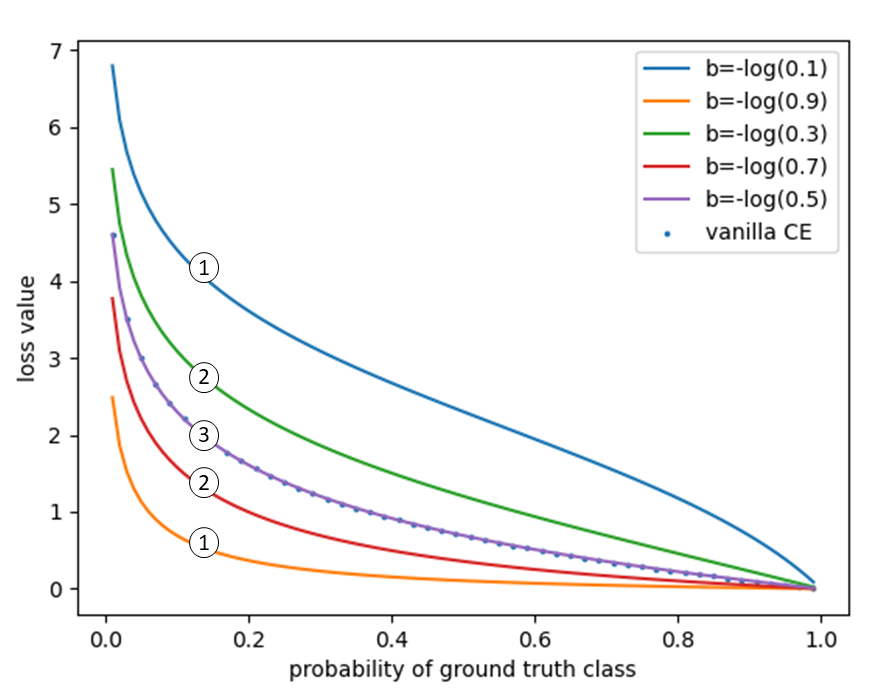
\includegraphics[width=0.9\columnwidth]{figure/lossdist} % Reduce the figure size so that it is slightly narrower than the column.
% 	\caption{The loss distribution for cross-entropy with our RTPB. This figure shows three pairs of loss with different resistance bias. In the pair \ding{172}, the resistance bias is set to be $-log(0.9)$ and $-log(0.1)$. And $-log(0.7)$ and $-log(0.1)$ is the bias value for the second pair, \ding{173}. In the last pair, \ding{174}, two classes take the same resistance bias value, and the loss value is equivalent to the vanilla CE. }
% 	\label{fig:loss}
% \end{figure}



Moreover, the loss value tends to be larger when the predicted distribution of $p_i$ in Eq. \eqref{eq:p_i} is close to the distribution of $e^{-b_i}= \frac{w_i^{a}}{\sum_{j \in \mathcal{C}_r} w_j^a}+ \epsilon$, which is correlated to the distribution of the predefined weight $\omega_i$ of each relationship in Eq. \eqref{eq:bias}. Because the distribution of $\omega_i$ correlates to the long-tail distribution of the training set, the resistance bias provides continuous supervision against the long-tailed distribution to avoid biased prediction.

%Besides, the RTB totally depends on the relative value difference of each class, and the exactly value dosen't matter because
%\begin{equation}
%	\hat{p_i}' = \frac{e^{z_{r_i}+b'}}{\sum_{j=0}^{N_r}e^{z_{r_j} + b'}} = \frac{e^\delta e^{z_{r_i}+b}}{e^\delta\sum_{j=0}^{N_r}e^{z_{r_j} + b}} = \hat{p_i} \label{eq:eq}
%\end{equation}
%Eq.\ref{eq:eq} shows that we change all the bias value with $b' = b + \delta$, its effect won't change when we use the softmax for classification.




% compare to re-weighting
% compare to margin

%\subsubsection{Gradient for RTB}
%With above bias value, the gradient of the classification score $z_{i}$ is:
%%\begin{equation}
%%	\frac{dL}{dz_i} = -\frac{1}{\sigma(z_i)} \frac{d\sigma(z_i)}{dz_i}=-\frac{1}{S_i}\frac{d\sigma(z_i)}{dz_i}
%%\end{equation}
%
%\begin{equation}
%	\frac{\partial \mathcal{\hat{L}}_i}{dz_j} = \frac{\partial \mathcal{\hat{L}}_i}{\partial (\hat{z}_j)} \frac{\partial (\hat{z}_j)}{\partial (z_j)}
%\end{equation}
%Because $\hat{z}_j = z_j + b_{s,o,j}$, the gradient turns to be:
%\begin{equation}
%	\begin{split}
%		\frac{\partial \mathcal{\hat{L}}_i}{\partial z_j} & = \frac{\partial \mathcal{\hat{L}}_i}{\partial (\hat{z}_j)} \times 1 = \sigma(\hat{\mathbf{Z}}_{s,o})_i - y_j \\
%		& = \frac{e^{b_j}p_j}{\sum_{k\in \mathcal{C}_r}e^{b_k} p_k} - y_j
%	\end{split}
%	\label{eq:grad_i}
%\end{equation}
%where $y_j= 1$ if $i=j$, otherwise $y_j = 0$. With Eq.\ref{eq:grad_i}, we can realize two point about the gradient value $\frac{\partial \mathcal{\hat{L}}_i}{\partial z_i}$. Firstly, for specific sample, the gradient turns to be closer to zero if the sample with larger RTB. Secondly, for a predicated result, there will be more significant gradient if the predicated distribution $\{p_j; j \in\mathcal{C}_r\}$ is similar to the distribution of the item $\{exp( b_{s,o,j});j \in\mathcal{C}_r\}$.
%Therefore, the RTB module encourages the model to predict a result the is opposite to the distribution of RTB.

\subsubsection{Objective with RTPB}
From another point of view, we can simply regard the $\hat{\mathbf{z}}_{s,o} = \mathbf{z}_{s,o} - \mathbf{b}$  as a joint to be optimized in the training phase and the result should be close to the baseline without RTPB. We then get the final prediction $ \mathbf{z}_{s,o} =\hat{\mathbf{z}}_{s,o} + \mathbf{b}$. In this manner, compared with the model without RTPB, we tend to judge the ambiguous predictions as belonging to another one with a larger resistance bias. Thus the classification boundary of two classes is tilted to the one with larger resistance. The tilt depends on the relative value relationship of resistance bias between the two relationship categories. For example, if we judge the label of a relationship as $i$, the $\hat{z}_{i}$ should outperform all of the rest $\{\hat{z}_j, j\neq i\}$ by a necessary classification margin $b_j - b_i$ .
% (for convenience, we ignore the influence of $\epsilon$ here)
% , which means the $p_i$ and $p_j$ should fit $p_i/e^{-b_i} > p_j/e^{-b_j}$.

